\documentclass[UTF8]{ctexart}

\usepackage{anyfontsize}
\usepackage{geometry}
    \geometry{left=4cm,right=4cm,top=2cm,bottom=2cm}
\usepackage{amsmath, amssymb, amsthm}
\usepackage{caption} 	 % 标题
\usepackage{xcolor} 	 % 颜色
\usepackage{graphicx} 	 % 引用图片
\usepackage{float}
\usepackage{multirow}
\usepackage{framed} 	 % 方框 \begin{framed}
\usepackage{indentfirst} 	 % 首行缩进 
    \setlength{\parindent}{0em}
\usepackage{setspace} 	 % 行间距 \begin{spacing}{arg}
\usepackage{extarrows} 	 % 箭头宏包 \xLongrightarrow 
\usepackage{esvect} 	 %向量箭头 \vv{}
\usepackage[version=3]{mhchem} 	 %化学方程式 \ce{}
\usepackage{siunitx} 	 %国际单位 \si{unit} \SI{number}{unit} 
\usepackage{array, makecell}
    \setcellgapes{5pt}

% font
\newcommand{\ve}[1]{\boldsymbol{\mathbf{#1}}}
\newcommand{\unit}[1]{\boldsymbol{\mathbf{\hat{#1}}}}
\newcommand{\mcal}{\mathcal}
\newcommand{\mscr}{\mathscr}
% common symbol
\newcommand{\E}{\mathrm e}
\renewcommand{\I}{\mathrm i}
\newcommand{\R}{\mathbb R}
\newcommand{\Z}{\mathbb Z}
\newcommand{\N}{\mathbb N}
\newcommand{\Q}{\mathbb Q}
\newcommand{\C}{\mathbb C}
% differentiation
\def \DD #1.#2.#3 {\dfrac{d^{#1} #2}{d #3^{#1}}}
\def \PP #1.#2.#3 {\dfrac{\partial^{#1} #2}{\partial #3^{#1}}}
\def \dd #1.#2 {\dfrac{d #1}{d #2}}
\def \pp #1.#2 {\dfrac{\partial #1}{\partial #2}} 
% matrix
\newcommand{\transp}{^{\top}}
\DeclareMathOperator{\tr}{tr}
% other command
\DeclareMathOperator{\Cov}{Cov}



\pagestyle{empty}

\begin{document}
\section{集合与概率}
\subsection{集合运算}
减法的等效形式:
\[ A \setminus B = A \setminus AB = A \cap \overline B \]
\begin{figure}[H]
     \centering
     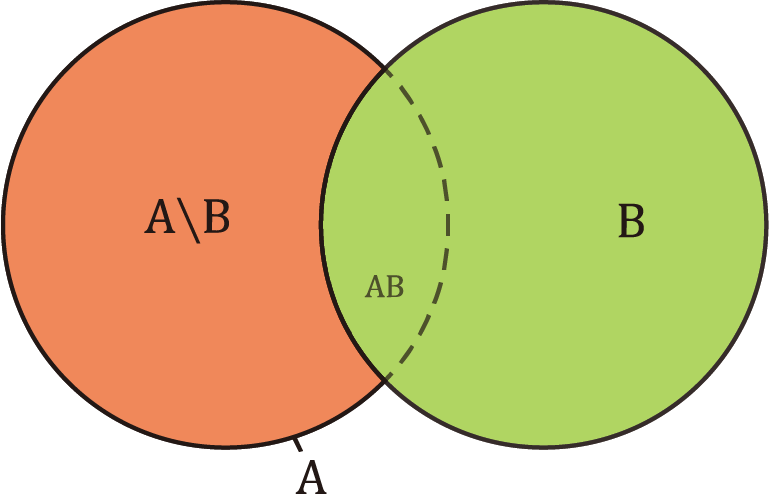
\includegraphics[width = 0.3\linewidth]{set_minus.png}
\end{figure}


\subsection{集合恒等式}
交换律, 结合律, 分配律略. 记全集为 $ U $,

幂等律:
\[ A \cup A = A  \]
\[ A \cap A = A \]

零元:
\[ A \cup U = U \]
\[ A \cap \varnothing = \varnothing \]

单位元:
\[ A \cup \varnothing = A \]
\[ A \cap U = A \]

吸收律:
\[ A \cup (A \cap B) = A \]
\[ A \cap (A \cup B) = A \]

若 $ A \subseteq A^+ $:
\[ A \cup A^+ = A^+ \]
\[ A \cap A^+ = A \]
即: 并集只可能增大集合,交集只可能减小集合

\subsection{概率运算}
减法公式:
\[ P(A \setminus B) = P(A \setminus AB) = P(A) - P(AB) \]

容斥原理:
\[ P(A \cup B) = P(A) + P(B) - P(A \cap B) \]

条件概率:
\[ P(A \mid B) = \dfrac{P(AB)}{P(B)} \]

乘法公式:
\[ P(AB) = P(A) P(B \mid A) = P(B) P(A \mid B) \]

全概率公式:
$ A_i \ (i = 1, \dots, n)$ 构成样本空间 $ \Omega $ 的完备事件组, 即 $ A_i $ 将 $ \Omega $ 有限划分.

\[ P(B) = \sum_i P(A_i) P(B | A_i) \]
\begin{figure}[H]
     \centering
     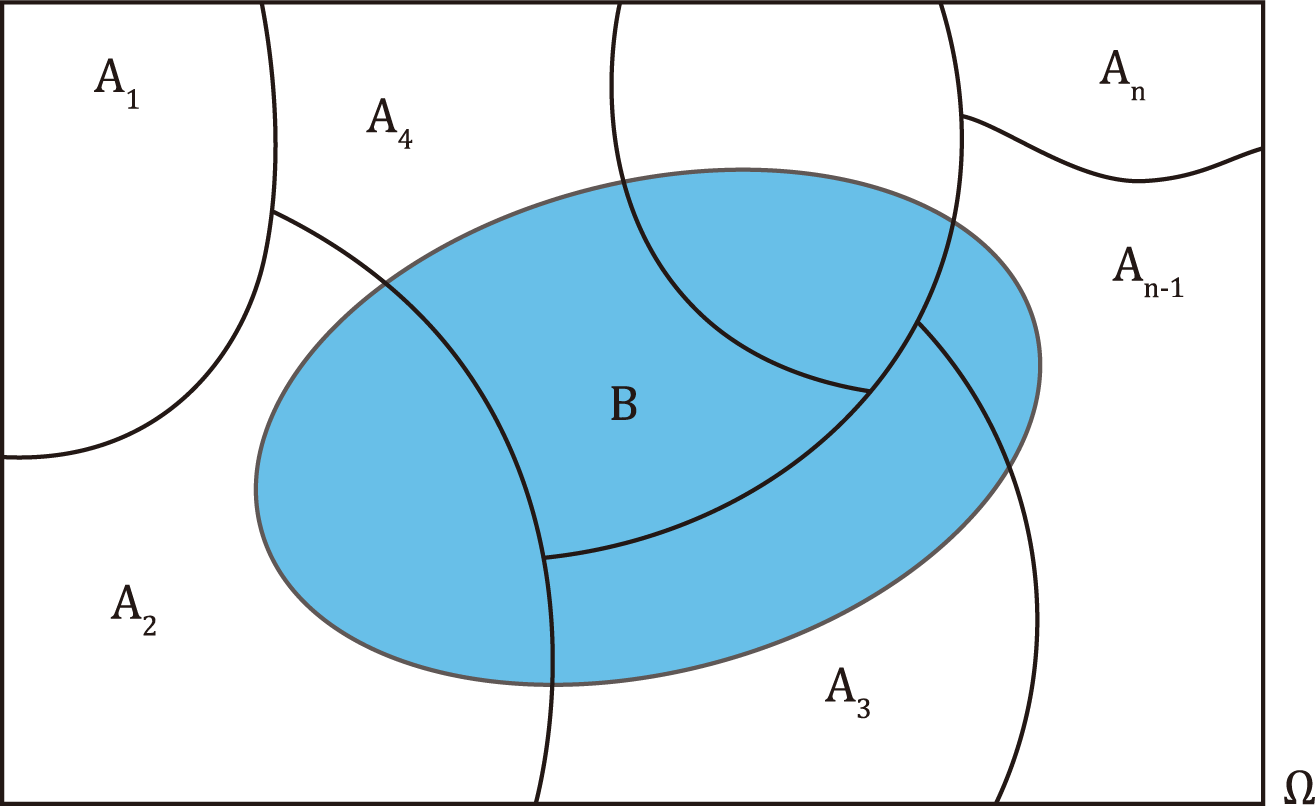
\includegraphics[width = 0.4\linewidth]{total_pro.png}
\end{figure}


贝叶斯公式:
\[ P(B_i \mid A) = \dfrac{P(AB_i)}{P(A)} = \dfrac{P(B_i) P( A \mid B_i)}{\sum\limits_i P(B_i) P(A \mid B_i)} \]

\subsection{独立与互斥}
互斥: 两事件不会同时发生, 即: $ A \cap B = \varnothing $.

独立: 一个事件的发生与否不影响另一个事件的发生, 即: $ P(AB) = P(A) P(B) $.

\newpage
\section{随机变量及其分布}
\subsection{一维}
连续:
\[ F_X(x) = P(X \leqslant x) = \int_{-\infty}^{x} f_X(t) \,dt \]
\[ f_X(x) = \dfrac{d}{dx}F_X(x) \]
\begin{figure}[H]
     \centering
     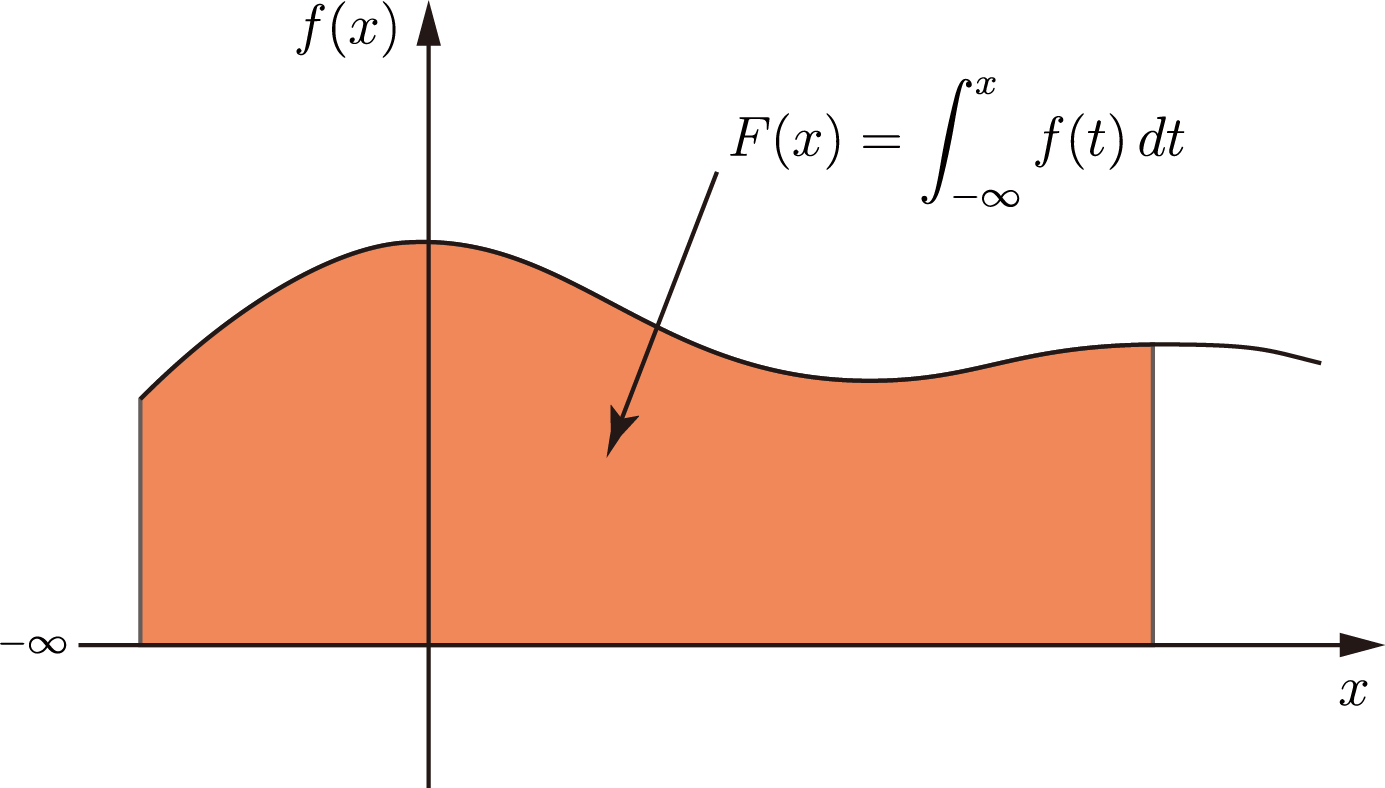
\includegraphics[width = 0.4\linewidth]{PDF&CDF.png}
\end{figure}

离散:
\[ F_X(x) = P(X \leqslant x) = \sum_{i \leqslant x} P(X = i) \]
\begin{figure}[H]
     \centering
     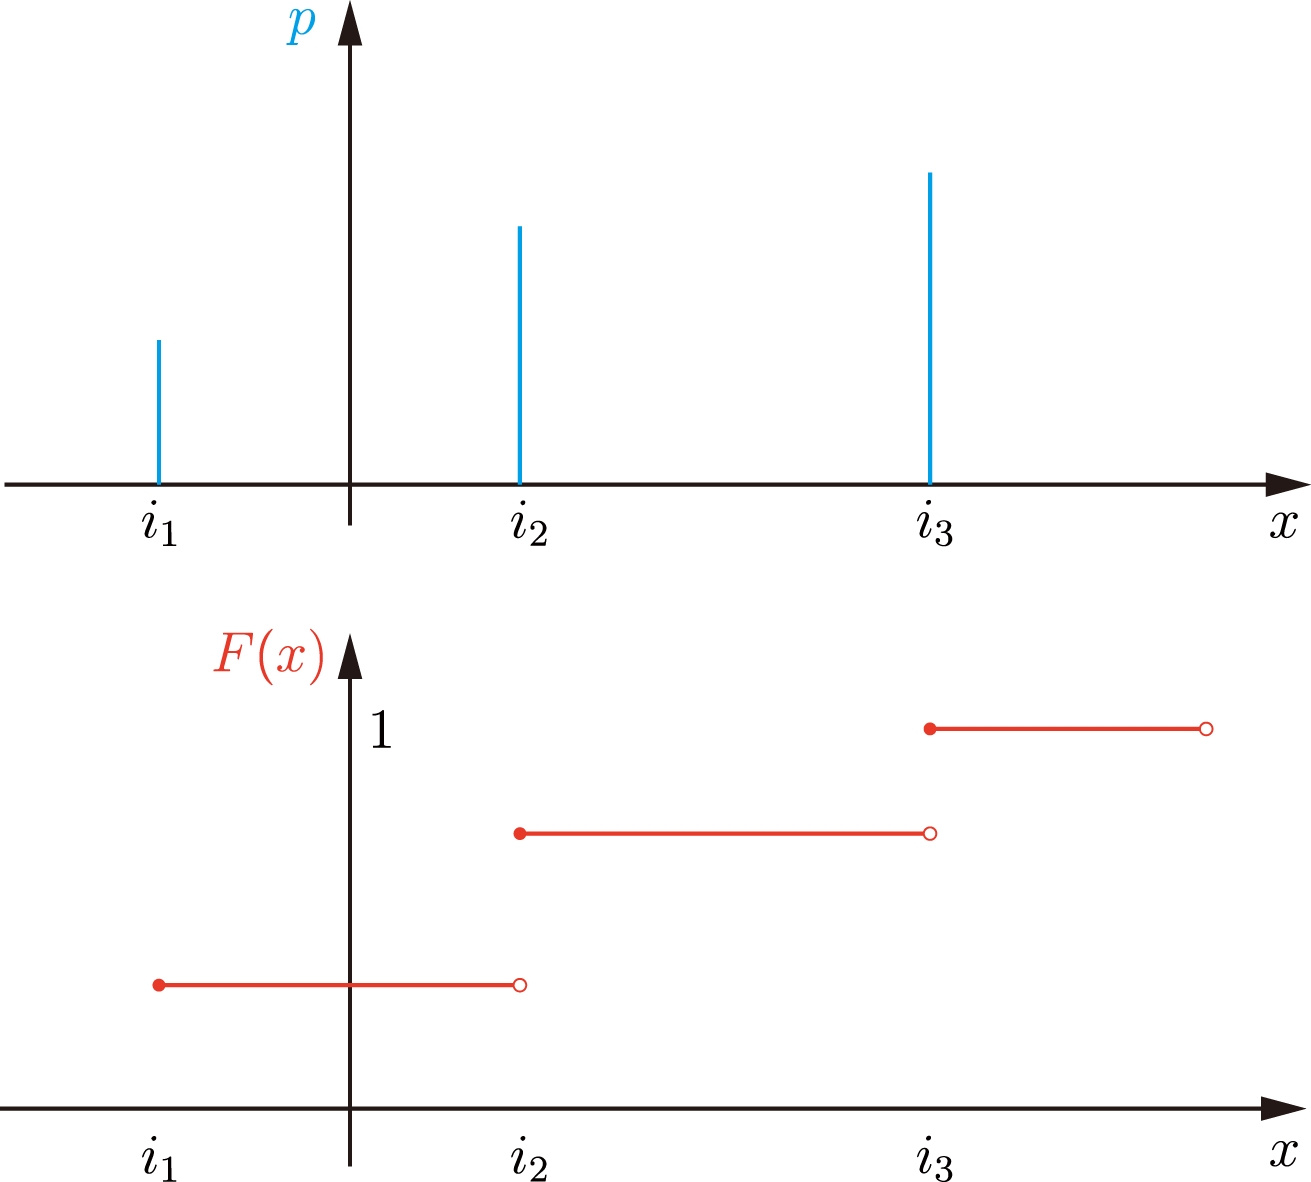
\includegraphics[width = 0.4\linewidth]{discrete_PDF&CDF.png}
\end{figure}


\subsection{二维}
\subsubsection{连续}
联合:
\[ F(x, y) = P(X \leqslant x, Y \leqslant y) = \int_{-\infty}^{x} \int_{-\infty}^{y} f(u, v) \,dv \,du \]
\[ f(x, y) = \dfrac{\partial^2 f}{\partial x \partial y} \]

边缘:
\[ F_X(x) = F(x, +\infty ) = P(X \leqslant x) = \int_{-\infty}^{x} f_X(t) \,dt \]
\[ f_X(x) = \int_{-\infty}^{+\infty} f(x, y) \,dy \]

\subsubsection{离散}
联合: \hskip 1em 记 $ p_{i j} = P(X = i, Y =j) $
\[ F(x, y) = P(X \leqslant x, Y \leqslant y) = \sum_{\substack{i \leqslant x \\ j \leqslant y}} p_{i j}  \]

边缘: \hskip 1em 记 $ p_{i \cdot} $ 表示 $ P(X = i) $ 而 $ Y $ 任意取值a 
\[ p_{i\cdot} = \sum\limits_j p_{i j} \]
\[ p_{\cdot j} = \sum\limits_i p_{i j} \]

\subsection{条件分布}
\[ F_{X \mid Y}(x \mid y) = P(X \leqslant x \mid Y = y) \]

离散:
\[ P(X = x_i \mid Y = y_j) = p_{i j} / p_{\cdot j} \]

连续:
\[ f_{X \mid Y}(x \mid y) = \dfrac{f(x, y)}{f_Y(y)} \]
\[ F_{X \mid Y}(x \mid y) = \int_{-\infty}^{x} f_{X \mid Y}(u \mid y) \,du \]

\subsection{独立}

\[ F(x, y) = F_X(x) F_Y(y) \Rightarrow \text{独立} \]
\[ \text{独立} \Leftrightarrow f(x, y) = f_X(x) f_Y(y) \]
\[ \text{独立} \Leftrightarrow p_{i j} = p_{i \cdot} p_{\cdot j} \]
\[ X, Y \text{ 独立} \Rightarrow f(X) \text{ 与 } g(Y) \text{ 也独立} \]


\section{随机变量的数字特征}
\subsection{期望}
离散:
\[ E(X) = \sum_{k = 1}^{\infty} x_k p_k \]
连续:
\[ E(X) = \int_{-\infty}^{+\infty} x f(x) \,dx \]

随机变量函数的期望:
\[ E(g(X)) = 
    \begin{cases}
        {\displaystyle \sum_{k = 1}^{\infty} g(x_k) p_k} \\[1em]
        {\displaystyle \int_{-\infty}^{+\infty} g(x) f(x) \,dx}
    \end{cases}
\]

性质:
\begin{itemize}
    \item 常数: $ E(C) = C $
    \item 线性: $ E(a X + b) = a E(X) + b $
    \item 若 $ X, Y $ 独立: $ E(XY) = E(X)E(Y) $
\end{itemize}


\subsection{方差}
\begin{itemize}
    \item 定义: $ D(X) = E[X - E(X)]^2 = E(X^2) - E(X)^2 $
    \item 常数: $ D(C) = 0 $
    \item 二次齐次, 平移不变性: $ D(a X + b) = a^2 D(X) $
    \item 加/减法: $ D(X \pm Y) = D(X) + D(Y) \pm 2\Cov(X, Y) $
    \item 协方差: $ D(X) = \Cov(X, X) $
\end{itemize}

\subsection{协方差}
\begin{itemize}
    \item 定义: $ \Cov(X, Y) = E\big[[X - E(X)][Y - E(Y)]\big] = E(X Y) - E(X) E(Y) $
    \item 交换律: $ \Cov(X, Y) = \Cov(Y, X) $
    \item 常数: $ \Cov(X, C) = 0 $
    \item 双线性: $ \Cov(a X + a', b Y + b') = ab \Cov(X, Y) $
    
    $ \qquad \Cov(X + Y, Z) = \Cov(X, Z) + \Cov(Y, Z) $
    \item $ X, Y $ 独立: $ \Cov(X, Y) = 0 $
\end{itemize}

协方差阵:
记 $ \sigma_{i j} = \Cov(X_i, X_j) $:
\[ \ve V = \begin{bmatrix}
    \sigma_{11} & \sigma_{12} & \cdots & \sigma_{1n} \\ 
    \sigma_{21} & \sigma_{22} & \cdots & \sigma_{2n} \\
    \vdots & \vdots & \ddots & \vdots \\
    \sigma_{n1} & \sigma_{n2} & \cdots & \sigma_{nn}
\end{bmatrix} \]

\subsection{相关系数}
\[ R(X, Y) = \dfrac{\Cov(X, Y)}{\sqrt{D(X)} \sqrt{D(Y)}} \]
性质:
\begin{itemize}
    \item $ |R(X, Y)| \leqslant 1 $
    \item $ |R(X, Y)| = 1 $ 的充要条件为: $ X $, $ Y $ 线性相关
    \item $ R(X, Y) = 0 $, $ X $, $ Y $ 没有线性关系(可能有其他相关关系)
\end{itemize}


\section{正态分布}
\subsection{标准正态分布}
\[ \varphi(x) = \dfrac{1}{\sqrt{2\pi}} \E^{-x^2 / 2} \]
\[ \Phi(x) = \int_{\infty}^{x} \varphi(t) \,dt \]
性质:

$ \Phi(0) = \dfrac{1}{2} $

$ \Phi(-x) = 1 - \Phi(x) $

\subsection{正态分布}
若 $ \dfrac{X - \mu}{\sigma} \sim N(0, 1) $, 则 $ X \sim N(\mu, \sigma^2) $. 此时对于 $ X $:

\[ f(x) = \dfrac{1}{\sqrt{2\pi} \sigma} \exp\left[ -\dfrac{(x - \mu)^2}{2\sigma^2} \right] \]
\[ F(x) = \Phi\left( \dfrac{x - \mu}{\sigma} \right) \]

\[ P(a < X \leqslant b) = \Phi\left( \dfrac{b - \mu}{\sigma} \right) - \Phi\left( \dfrac{a - \mu}{\sigma} \right) \]

\subsection{正态分布性质}
$ X \sim N(\mu, \sigma^2) $, $ Y_i \sim N(\mu_i, \sigma_i^2) $:
\begin{itemize}
    \item $ E(X) = \mu $, $ D(X) = \sigma^2 $
    \item $ a X + b \sim N(a \mu + b, a^2 \sigma^2) $
    \item $ Y_1 \pm Y_2 \sim N(\mu_1 \pm \mu_2, \sigma_1^2 + \sigma_2^2) \qquad (\text{注意方差总是相加}) $ 
\end{itemize}


\section{大数定律与中心极限定理}
\subsection{切比雪夫不等式}
\[ P\big( |X - E(X)| < \varepsilon \big) \geqslant 1 - \dfrac{D(X)}{\varepsilon^2} \]

由此推导出:

随机变量序列 $ E(X_n) = \mu_n $, $ D(X_n) = \sigma_n^2 $, $ \lim\limits_{n \to \infty} \sigma_n^2 = 0 $, 则:
\[ X_n \xlongrightarrow{P} \mu_n \]

\subsection{大数定律}
\subsubsection{切比雪夫大数律}
\underline{\textbf{独立}}随机变量序列 $ \{ X_k \} $, $ X_k $ 的期望方差均存在且\underline{\textbf{方差有界}}, 则:
\[ \dfrac{1}{n} \sum_{k = 1}^{n} X_k - \dfrac{1}{n} \sum_{k = 1}^{n} E(X_k) \xlongrightarrow{P} 0  \]

\subsubsection{独立同分布大数律}
$ \{ X_k \} $ \underline{\textbf{独立同分布}}, $ E(X_k) = \mu $, $ D(X_k) = \sigma^2 $:
\[ \overline{X} \xlongrightarrow{P} \mu \]


\subsection{中心极限定理}
\subsubsection{独立同分布}
随机变量序列 $ \{X_k\} $ \underline{\textbf{独立同分布}}, $ E(X_k) =\mu_k $, $ D(X_k) = \sigma^2 $. 
\vskip 0.5em
\begin{spacing}{2}
则随机变量 $ Y_n = \dfrac{\sum\limits_{k = 1}^{n} X_k - n\mu}{\sqrt n \sigma} = \dfrac{\dfrac{1}{n} \sum\limits_{k = 1}^{n} X_k - \mu}{\sigma / \sqrt n} $ 当 $ n \to \infty $ 时的极限分布函数为标准正态分布函数 $ \Phi(x) $. 
\end{spacing}
即意味着, 当 $ n $ 充分大:
\[ \sum_{k = 1}^{n} X_k  \ \dot\sim\ N(n\mu, n\sigma^2)  \]
\[ \overline X = \dfrac{1}{n}\sum_{k = 1}^{n} X_k \ \dot\sim \ N\left(\mu, \dfrac{\sigma^2}{n}\right) \]

\section{数理统计}
\subsection{三大分布}
\subsubsection{$ \chi^2 $ 分布}
$ X_1, \dots, X_n $ 独立同服从 $ N(0, 1) $, 称随机变量 $ \chi^2 = \sum\limits_{i = 1}^{n} X_i^2 $ 服从自由度为 $ n $ 的 $ \chi^2 $ 分布, 记作:
\[ \chi^2 \sim \chi^2 (n) \]

性质:
\begin{enumerate}
    \item $ \chi^2 (n) = \Gamma\left( \dfrac n 2, \dfrac 1 2 \right) $
    \item $ \chi_1^2 \sim \chi^2(n) $, $ \chi_2^2 \sim \chi^2(m) $, $ \chi_1 $, $ \chi_2 $ 独立, 则 $ \chi_1^2  + \chi_2^2 \sim \chi^2 (n + m) $
\end{enumerate}

\begin{figure}[H]
     \centering
     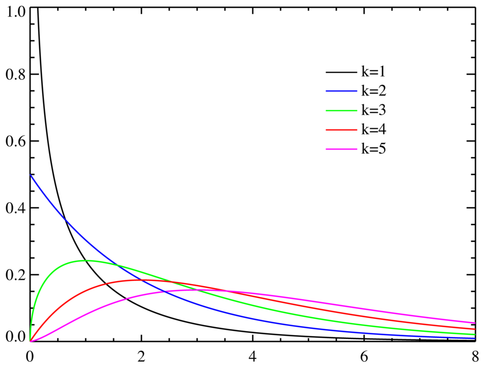
\includegraphics[width = 0.45\linewidth]{Chi-square_distributionPDF}
\end{figure}



\subsubsection{$ t $ 分布}
$ X \sim N(0, 1) $, $ Y \sim \chi^2(n) $, $ X $, $ Y $ 独立:
\[ t = \dfrac{X}{\sqrt{Y / n}} \sim t(n) \]
称 $ t(n) $ 自由度为 $ n $
\vskip 1em

性质:
\begin{enumerate}
    \item $ n \to \infty $, 则 $ t(n) \to N(0, 1) $
\end{enumerate}

\begin{figure}[H]
     \centering
     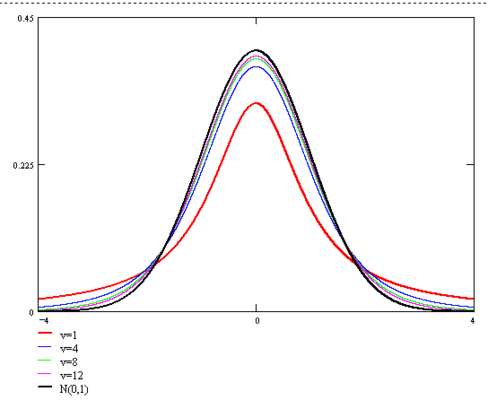
\includegraphics[width = 0.45\linewidth]{TStudent}
\end{figure}


\subsubsection{$ F $ 分布}
$ X_1 \sim \chi^2 (n_1) $, $ X_2 \sim \chi^2 (n_2) $, $ X_1 $, $ X_2 $ 独立:
\[ F = \dfrac{X_1 / n_1}{X_2 / n_2} \sim F(n_1, n_2) \]
称 $ F(n_1, n_2) $ 自由度为 $ (n_1, n_2) $. $ F $ 分布的图形与 $ \chi^2 $ 分布类似.
\vskip 1em

性质:
\begin{enumerate}
    \item $ F \sim F(n_1, n_2) $, 则 $ \dfrac{1}{F} \sim F(n_2, n_1) $
    \item $ X \sim t(n) $, 则 $ X^2 \sim F(1, n) $
\end{enumerate}

\subsubsection{分位点}
若有: $ F(x_p) = P(X \leqslant x_p ) = p $, 则称 $ x_p $ 为分布 $ F $ 的 $ p $ 分位点:


\begin{enumerate}
    \item 标准正态分布密度函数为偶函数 $ u_p + u_{1 - p} = 0 $
    \item 当 $ n > 45 $ 时, $ \chi^2 $ 分布分位点: $ \chi_p^2(n) \approx (u_p + \sqrt{2n - 1})^2 / 2 $
    \item $ t $ 分布与标准正态分布密度函数近似: $ - t_p = t_{1 - p} $
    \item $ F $ 分布有: $ F_p(n_1, n_2) = \dfrac{1}{F_{1 - p} (n_2, n_1)} $
\end{enumerate}


\subsection{统计量}
样本均值:
\[ \overline X = \frac 1 n \sum_{i = 1}^{n} X_i \]

样本方差:
\[ S^2 = \dfrac{1}{n - 1} \sum^{n}_{i = 1} (X_i - \overline X)^2 = \dfrac{1}{n - 1} \left( \sum_{i = 1}^n X_i^2 - n \overline X^2 \right)  \]

样本标准差: $ S = \sqrt{S^2} $
\vskip 1em

样本 $ k $ 阶(原点)矩:
\[ A_k = \dfrac{1}{n} \sum_{i = 1}^{n} X_i^k \]

样本 $ k $ 阶中心距:
\[ B_k = \dfrac{1}{n} \sum_{i = 1}^{n} (X_i - \overline X)^k \]

恒等式:
\[ B_2 = A_2 - \overline X^2 \]
\[ S^2 = \dfrac{n}{n - 1} B_2 \]

\subsection{抽样分布定理}
\subsubsection{一个正态分布总体}
样本均值的分布:
$ X_1, X_2, \dots, X_n $ 来自总体 $ N(\mu, \sigma^2) $, 则:
\[ {\color{red} \overline{X}} \sim N\left( \mu, \dfrac{\sigma^2}{n} \right)  \hspace{3em} \dfrac{{\color{red} \overline X} - \mu}{\sigma / \sqrt{n}} \sim N(0, 1) \]

样本方差和 $ 2 $ 阶中心距的分布:
\[ \dfrac{(n - 1) {\color{red} S^2}}{\sigma^2} = \dfrac{n {\color{red} B_2}}{\sigma^2} \sim \chi^2(n - 1) \]

标准差的分布与样本均值:
\[ \dfrac{{\color{red} \overline{X}} - \mu}{ {\color{red} S} / \sqrt n} \sim t(n - 1) \]

\subsubsection{任意总体}
$ X_1, \dots, X_n $ 来自任何总体:
\[ E(\overline X) = E(X) \hspace{3em} D(\overline X) = \dfrac{D(X)}{n} \]
中心极限定理: 当 $ n $ 充分大时, 近似有
\[ \dfrac{{\color{red} \overline{X}} - \mu}{\sigma / \sqrt n} \ \dot\sim\ N(0, 1) \]
\[ \dfrac{{\color{red} \overline{X}} - \mu}{S / \sqrt n} \ \dot\sim\ N(0, 1) \]

\section{点估计}
\subsection{矩估计法}
\subsection{极大似然估计法}
似然函数:\[ L(\theta) = \prod_{i = 1}^{n} p(x_i, \theta) \text{  或  } L(\theta) = \prod_{i = 1}^n f(x_i, \theta) \]

要使似然函数取得最大值, 即求满足似然方程的 $ \theta $:
\[ \dd L(\theta).{\theta} = 0 \]

上式等价于
\[ \dd {\ln L(\theta)}.{\theta} = 0 \]


\subsection{估计量的评选标准}
\subsubsection{无偏性}
若估计量 $ \hat \theta $ 的期望等于被估计的参数, 则称 $ \hat \theta $ 为无偏估计量, 否则为有偏估计量.
\[ E(\hat \theta) = \theta \]

对有偏估计量 $ \hat \theta $, 记 $ b(\hat \theta) = E(\hat\theta) - \theta $. 若:
\[ \lim_{n \to \infty} b(\hat \theta) = 0 \]

则称 $ \hat \theta $ 为渐进无偏估计量.

\paragraph{常见无偏估计量}
若总体 $ X $ 服从任意分布, 则样本均值 $ \overline X $, 样本 $ k $ 阶矩 $ A_k $, 样本方差 $ S^2 $ 分别是 $ E(X) $, $ E(X^k) $, $ D(X) $ 的无偏估计量.

\subsubsection{有效性}
设 $ \hat \theta_1 $ 和 $ \hat \theta_2 $ 为两个无偏估计量, 若:
\[ D(\hat \theta_1) \leqslant D(\hat \theta_2) \]

则称 $ \hat \theta_1 $ 比 $ \hat \theta_2 $ 更有效.


\section{区间估计}
\subsection{一个正态总体}
总体 $ X \sim N(\mu, \sigma^2) $, $ X_1, \dots, X_n $ 是来自总体的样本:
\subsubsection{已知 $ \sigma^2 = \sigma_0^2 $, 求 $ \mu $ 的置信区间}
取样本函数:
\[ \dfrac{\overline X - {\color{red} \mu}}{\sigma_0 / \sqrt n} \sim N(0, 1) \]

\subsubsection{$ \sigma^2 $ 未知, 求 $ \mu $ 的置信区间}
取样本函数:
\[ \dfrac{\overline X - {\color{red} \mu}}{S / \sqrt n} \sim t(n - 1) \]

\subsubsection{$ \mu $ 未知, 求 $ \sigma^2  $ 的置信区间}
取样本函数:
\[ \dfrac{(n - 1) S^2}{\color{red} \sigma^2} \sim \chi^2(n - 1) \]



\section{假设检验}
\subsection{一个正态总体均值假设检验表}
\renewcommand{\arraystretch}{1.5}
\begin{table}[H]
\centering
\makegapedcells
\begin{tabular}{c|c|c|c}
    \hline
    \multirow{2}{*}{$ H_0 $} & \multirow{2}{*}{$ H_1 $} & $ \sigma^2 $ 已知 & $ \sigma^2 $ 未知 \\ \cline{3-4} 
    &                   & \multicolumn{2}{c}{显著性水平 $ \alpha $ 下 $ H_0 $ 的拒绝域} \\ \hline
    $ \mu = \mu_0 $ & $ \mu \neq \mu_0 $ & $ |U| > u_{1 - \frac{\alpha}{2}} $ & $ |t| > t_{1 - \frac{\alpha}{2}} $ \\ \hline
    $ \mu = \mu_0 $ & $ \mu > \mu_0 $ & $ U > u_{1 - \alpha} $ & $ t > t_{1 - \alpha}(n - 1) $ \\ \hline
    $ \mu = \mu_0 $ & $ \mu < \mu_0 $ & $ U < u_{\alpha} $ & $ t < t_{\alpha}(n - 1) $ \\ \hline
    \end{tabular}
\end{table}



\subsection{一个正态总体方差假设检验表}
\renewcommand{\arraystretch}{1.5}
\begin{table}[H]
\centering
\makegapedcells
\begin{tabular}{c|c|c}
    \hline
    $ H_0 $ & $ H_1 $ & $ \mu $ 未知, 显著性水平 $ \alpha $ 下 $ H_0 $ 的拒绝域 \\

    \hline
    $ \sigma^2 = \sigma_0^2 $ & $ \sigma^2 \neq \sigma_0^2 $ & $ \chi^2 < \chi_{\alpha / 2}^2(n - 1) $ 或 $ \chi^2 > \chi_{1 - \frac{\alpha}{2}}^2 (n - 1) $ \\

    \hline
    $ \sigma^2 = \sigma_0^2 $ & $ \sigma^2 > \sigma_0^2 $ & $ \chi^2 > \chi_{1 - \alpha}^2 (n - 1) $ \\

    \hline
    $ \sigma^2 = \sigma_0^2 $ & $ \sigma^2 < \sigma_0^2 $ & $ \chi^2 <  \chi_{\alpha}^2 (n - 1) $ \\

    \hline
    \end{tabular}
\end{table}

下图从上到下依次为双侧检验, 左侧检验, 右侧检验的图示:
\begin{figure}[H]
    \centering
    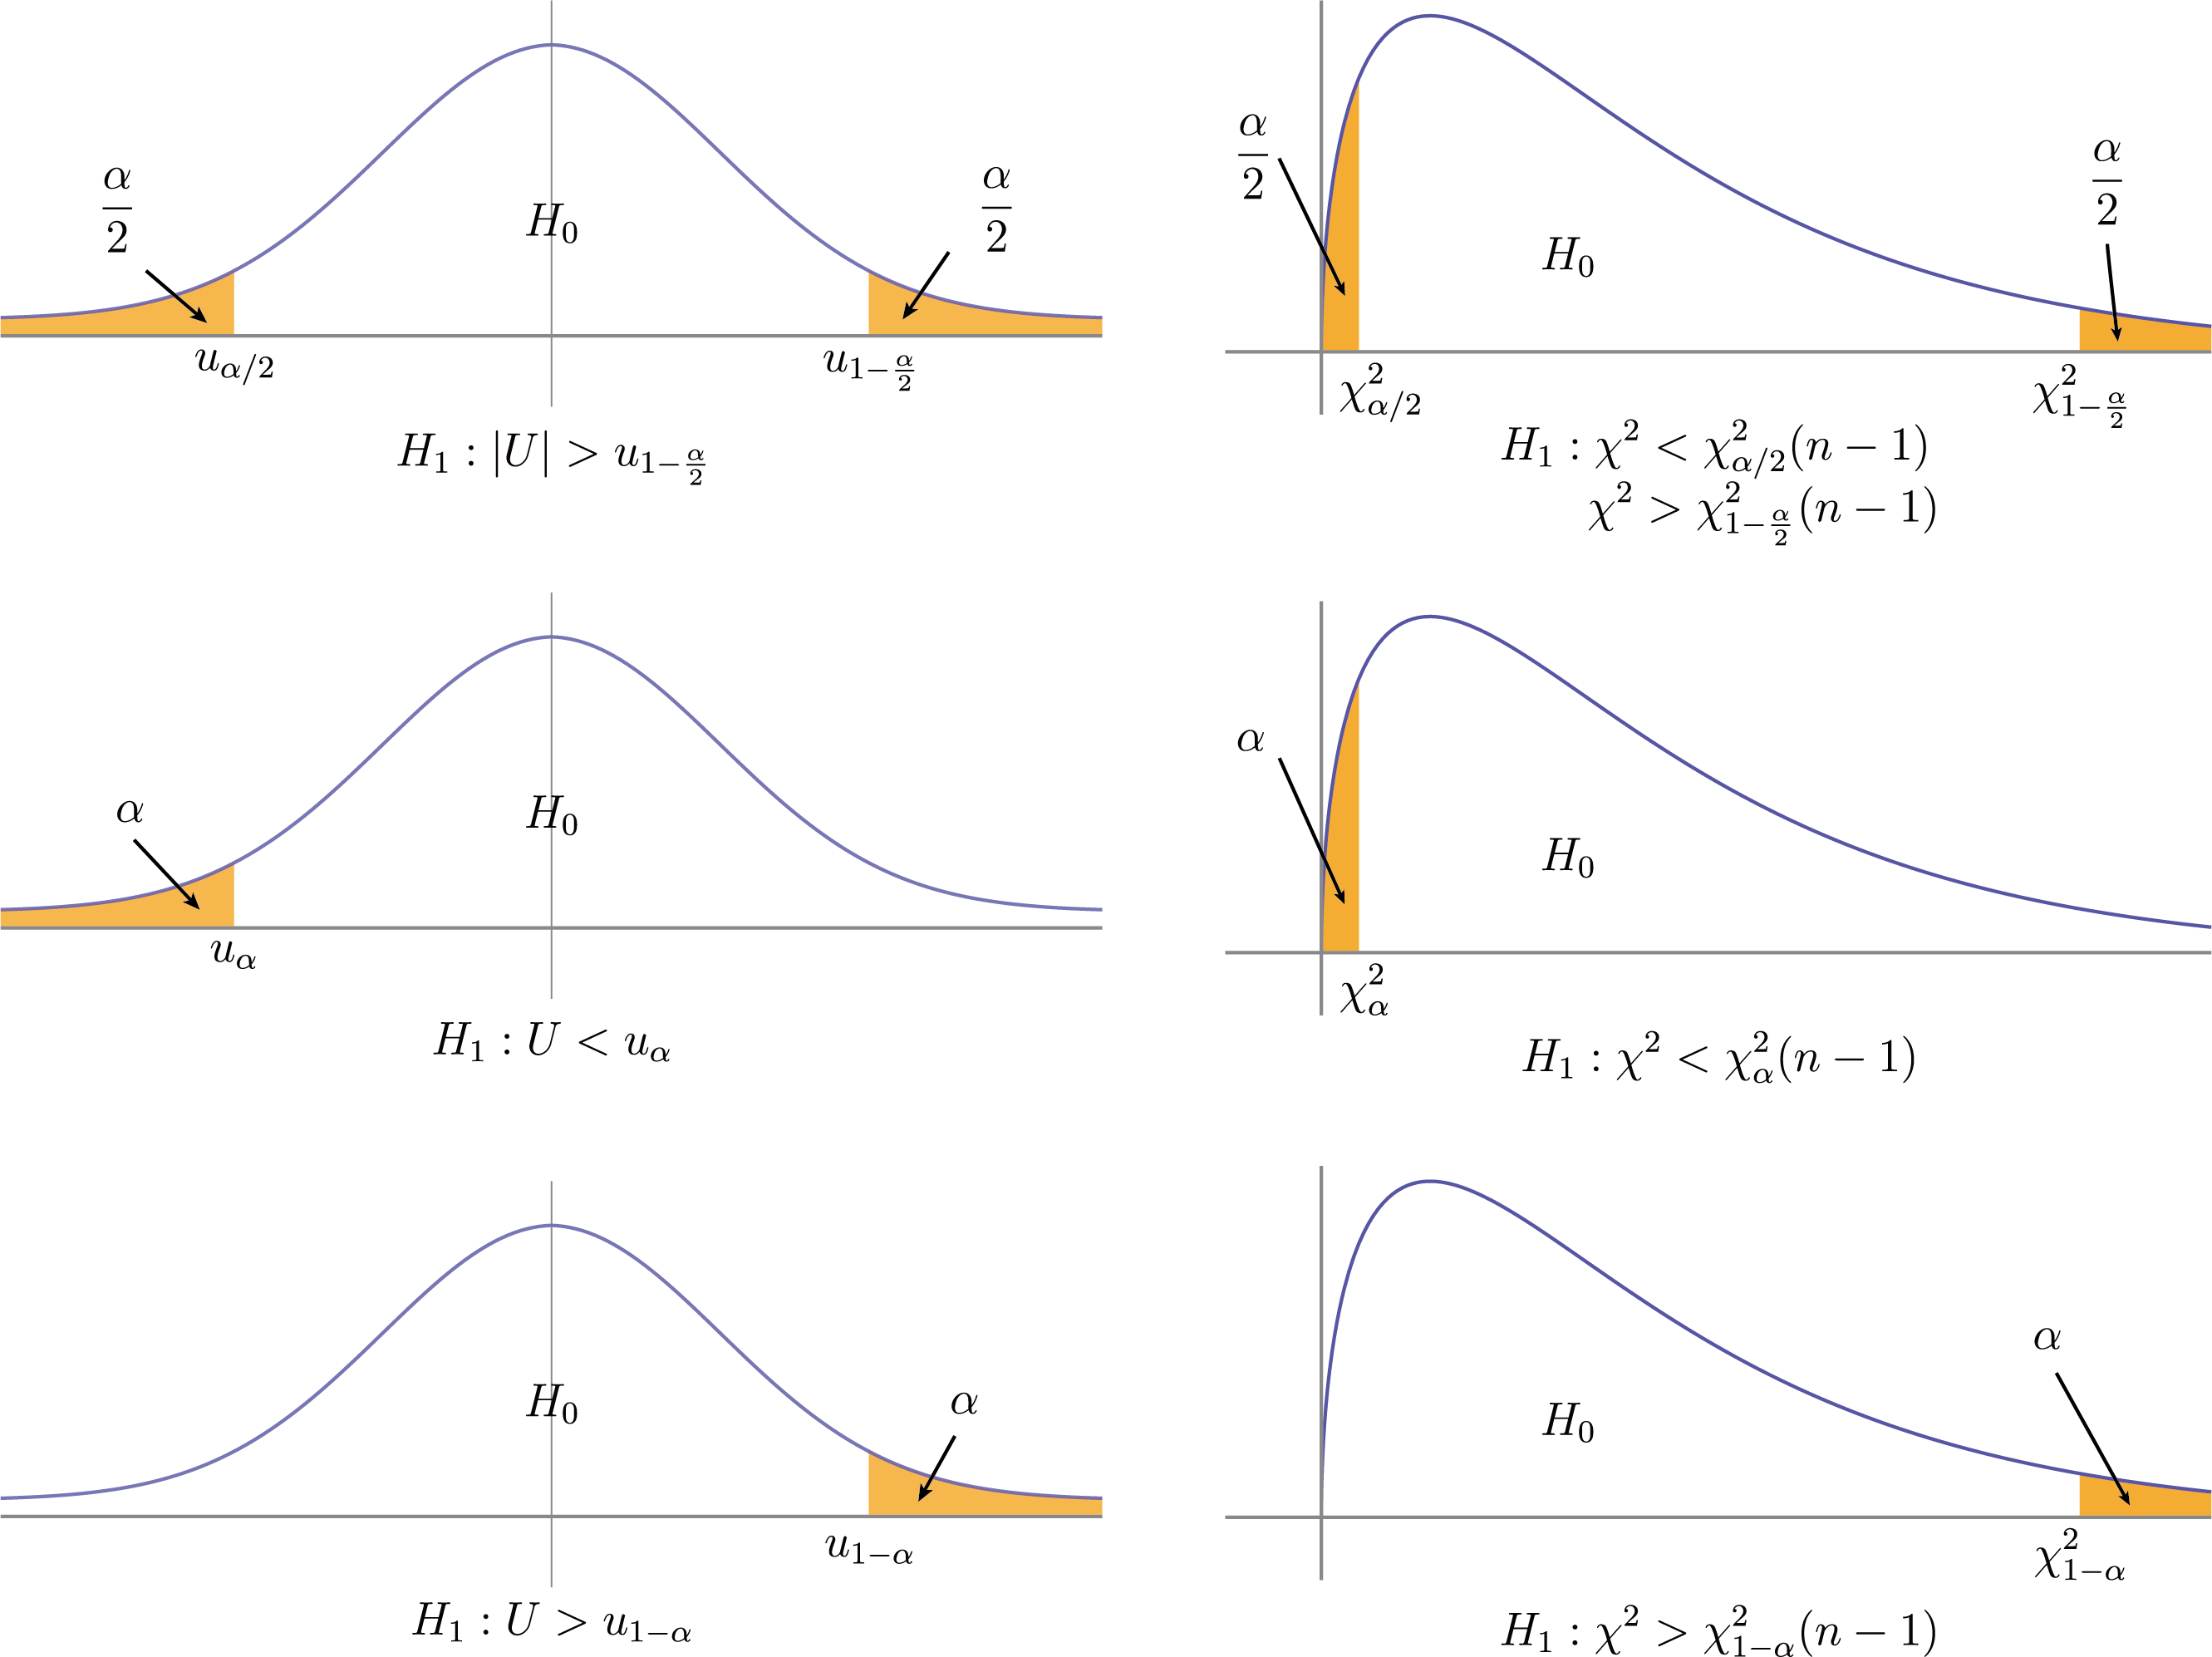
\includegraphics[width = 0.85\linewidth]{confidence_interval}
    \caption*{\textit{$ u $ 和 $ \chi^2 $ 检验: 黄色部分为拒绝域 $ H_1 $}}
\end{figure}

$ t $ 分布概率密度函数图像与标准正态分布相似, $ t $ 检验可参考 $ u $ 检验.




\newpage
\section{离散型模型}
\renewcommand{\arraystretch}{2.5}
\begin{table}[H]
\centering
\makegapedcells
\begin{tabular}{c|c|c|c|c}
    \hline
    名称 & 记号/参数 & 概率 & 期望 & 方差 \\

    \hline
    二项分布 & $ B(n, k) $ & $ p_k = \binom n k p^k (1 - p)^{n - k} $ & $ n p $ & $ n p (1 - p) $ \\

    \hline
    几何分布 & $ G(p) $ & $ p_k = p q^{k - 1} $ & $ \dfrac{1}{p} $ & $ \dfrac{1 - p}{p^2} $ \\
    
    \hline
    超几何分布 & $ H(n, M, N) $ & $ p_k = \dfrac{\binom{M}{k} \binom{N - M}{n - k}}{\binom{N}{n}} $ & $ n \dfrac{M}{N} $ & $ n \dfrac{M}{N} \left( 1 - \dfrac{M}{N} \right) \dfrac{N - n}{N - 1} $ \\

    \hline
    泊松分布 & $ P(\lambda) $ & $ p_k = \dfrac{\lambda^k}{k!} \E^{-\lambda} $ & $ \lambda $ & $ \lambda $ \\

    \hline
\end{tabular}
\end{table}

\section{连续型模型}
\renewcommand{\arraystretch}{2.5}
\begin{table}[H]
\centering
\makegapedcells
\begin{tabular}{c|c|c|c|c}
    \hline
    名称 & 记号/参数 & 密度函数 & 期望 & 方差 \\

    \hline
    均匀分布 & $ U(a, b), U(G) $ & $ f(x) = \begin{cases}
        \dfrac{1}{m(G)} = \dfrac{1}{b - a} &, x \in (a, b) \\
        0 &, x \notin (a,b) 
    \end{cases} $ & $ \dfrac{a + b}{2} $ & $ \dfrac{(b - a)^2}{12} $ \\

    \hline
    $ \Gamma $ 分布 & $ \Gamma(\alpha, \beta) $ & $ f(x) = \begin{cases}
        \dfrac{\beta^\alpha}{\Gamma(\alpha)} x^{\alpha - 1} \E^{-\beta x} &, x > 0 \\
        0 &, x \leqslant 0
    \end{cases}  $ & $ \dfrac{\alpha}{\beta} $ & $ \dfrac{\alpha}{\beta^2} $ \\

    \hline
    指数分布 & $ e(\beta) = \Gamma(1, \beta) $ & 
        $ \begin{array}{c}
            f(x) = 
        \beta \E^{-\beta x} \quad, x > 0 \\
        F(x) = 1 - \E^{- \beta x} \quad, x > 0
        \end{array} $
        & $ \dfrac{1}{\beta} $ & $ \dfrac{1}{\beta^2} $ \\

    \hline
    $ \chi^2 $ 分布 & $ \chi^2(n) $ & $ f(x) = \begin{cases}
        \dfrac{x^{n / 2 - 1} \E^{-x / 2}}{2^{n / 2} \Gamma(n / 2)}  &, x > 0 \\
        0 &, x \leqslant 0
    \end{cases}  $ & $ n $ & $ 2 n $ \\

    \hline
\end{tabular}
\end{table}


\end{document}